 % The main file for CAMP reports
 % Don't put any content in here. 
 % Don't even include content files by using \input or \inlcude. 
 % Put your content to TEXT.TEX or include it there using \input.
 % Uses:
 %		SETTINGS.TEX	contains the settings for this document
 %		COMMANDS.TEX	contains commands which can be used while writing
 %		INFO.TEX			contains the author, title and so on for the cover
 %		COVER.TEX			formats the front cover of the document
 %		ABSTRACT.TEX	contains the abstract to be included (if needed)
 %		TEXT.TEX			contains the actual content of the document
 %		BIB.BIB				containt the BibTeX entries for the document
 
 
%% Draft document mode
%% Final document
\documentclass[11pt,a4paper,bibtotoc,idxtotoc,headsepline,footsepline,footexclude,BCOR12mm,DIV13]{scrbook}

%\documentclass[11pt,a4paper,bibtotoc,idxtotoc,headsepline,footsepline,footexclude,BCOR20mm,DIV10]{scrbook}

% KOMA-Optionen:
%  bibtotoc: include bibliography in table of contents
%  idxtotoc: include index in table of contents
%  headsepline: use horizontalline under heading
%  BCOR: binding correcion (Bindungskorrektur) (e.g.: BCOR5mm)
%  DIV: Number of sheet sections (used for layout) (e.g.: DIV12) 



% include title and author information for the cover
% Set here the title, authors and other stuff to be used for the cover
% This file is used by MAIN.TEX

% set title, authors and stuff for the cover
\def\doctype{Diplomarbeit in Informatik}
\def\title{Semi-automated detection of sanitization, autehntication and declassification errors in UML state charts}
\def\titleGer{Halbautomatische Erkennung von Sanitisierungs-, Authenifizierungs- und Deklassifierungsfehlern in UM L-Zusantsdiagrammen}
\def\author{Md Adnan Hossain Rabbi}
\def\date{November 15, 2015}

% text to appear in the footer
\def\footertext{}

% include settings
% Included by MAIN.TEX
% Defines the settings for the CAMP report document

\renewcommand{\sectfont}{\normalfont \bfseries}        % Schriftart der Kopfzeile

% manipulate footer
\usepackage{scrpage2}
\pagestyle{scrheadings}
\ifoot[\footertext]{\footertext} % \footertext set in INFO.TEX
%\setkomafont{pagehead}{\normalfont\rmfamily}
\setkomafont{pagenumber}{\normalfont\rmfamily}

%% allow sophisticated control structures
\usepackage{ifthen}

% use Palatino as default font
\usepackage{palatino}

% enable special PostScript fonts
\usepackage{pifont}

% make thumbnails
\usepackage{thumbpdf}

%to use the subfigures
\usepackage{subfigure}


\usepackage{colortbl}


%% show program code\ldots
%\usepackage{verbatim}
%\usepackage{program}

%% enable TUM symbols on title page
\usepackage{styles/tumlogo}
\usepackage{url}

\usepackage{multirow}

%% use colors
\usepackage{color}

%% make fancy math
\usepackage{amsmath}
\usepackage{amsfonts}
\usepackage{amssymb}
\usepackage{textcomp}
\usepackage{yhmath} % f�r die adots 
%% mark text as preliminary
%\usepackage[draft,german,scrtime]{prelim2e}

%% create an index
\usepackage{makeidx}

% for the program environment
\usepackage{float}

%% load german babel package for german abstract
%\usepackage[german,american]{babel}
\usepackage[german,english]{babel}
\selectlanguage{english}

% use german characters as well
\usepackage[latin1]{inputenc}       % allow Latin1 characters

% use initals dropped caps - doesn't work with PDF
%\usepackage{dropping}


\usepackage{styles/shortoverview}
%----------------------------------------------------
%      Graphics and Hyperlinks
%----------------------------------------------------

%% check for pdfTeX
\ifx\pdftexversion\undefined
 %% use PostScript graphics
 \usepackage[dvips]{graphicx}
 \DeclareGraphicsExtensions{.eps,.epsi}
 \graphicspath{{figures/}{figures/review}} 
 %% allow rotations
 \usepackage{rotating}
 %% mark pages as draft copies
 %\usepackage[english,all,light]{draftcopy}
 %% use hypertex version of hyperref
 \usepackage[hypertex,hyperindex=false,colorlinks=false]{hyperref}
\else %% reduce output size \pdfcompresslevel=9
 %% declare pdfinfo
 %\pdfinfo { 
 %  /Title (my title) 
 %  /Creator (pdfLaTeX) 
 %  /Author (my name) 
 %  /Subject (my subject	) 
 %  /Keywords (my keywords)
 %}
 %% use pdf or jpg graphics
 \usepackage[pdftex]{graphicx}
 \DeclareGraphicsExtensions{.jpg,.JPG,.png,.pdf,.eps}
 \graphicspath{{figures/}} 
 
 %% Load float package, for enabling floating extensions
 \usepackage{float}
 
 %% allow rotations
 \usepackage{rotating}
 %% use pdftex version of hyperref
 \usepackage[pdftex,colorlinks=true,linkcolor=red,citecolor=red,%
 anchorcolor=red,urlcolor=red,bookmarks=true,%
 bookmarksopen=true,bookmarksopenlevel=0,plainpages=false%
 bookmarksnumbered=true,hyperindex=false,pdfstartview=%
 ]{hyperref}
%
%\usepackage[pdftex,colorlinks=false,linkcolor=red,citecolor=red,%
% anchorcolor=red,urlcolor=red,bookmarks=true,%
% bookmarksopen=true,bookmarksopenlevel=0,plainpages=false%
% bookmarksnumbered=true,hyperindex=false,pdfstartview=%
% ]{hyperref}
\fi




%% Fancy chapters
%\usepackage[Lenny]{fncychap}
%\usepackage[Glenn]{fncychap}
%\usepackage[Bjarne]{fncychap}

%\usepackage[avantgarde]{quotchap}

% set the bibliography style
%\bibliographystyle{styles/bauermaNum}
%\bibliographystyle{alpha}
\bibliographystyle{plain}

% include commands
% Commands to be used within the TUM report document
% Included by MAIN.TEX
% Please include your own cool commands here. 
% Be only sure to comment it sufficiently so others can use it.

%-------------------------------------------------------------
%                      Own Commands
%-------------------------------------------------------------


%-------------------------------------------------------------
% math stuff -------------------------------------------------

% nice R, N, C
\newcommand{\nat}{\mathbb{N}}
\newcommand{\real}{\mathbb{R}}
\newcommand{\compl}{\mathbb{C}}



% norm
\newcommand{\norm}[1]{\left\| #1 \right\|}

% un demi
\newcommand{\half}{\frac{1}{2}}

% parantheses
\newcommand{\parenth}[1]{ \left( #1 \right) }
\newcommand{\bracket}[1]{ \left[ #1 \right] }
\newcommand{\accolade}[1]{ \left\{ #1 \right\} }
%\newcommand{\angle}[1]{ \left\langle  #1 \right\rangle }

% partial derivative: %#1 function, #2 which variable
% simple / single line version
\newcommand{\pardevS}[2]{ \delta_{#1} f(#2) }
% fraction version
\newcommand{\pardevF}[2]{ \frac{\partial #1}{\partial #2} }

% render vectors: 3 and 4 dimensional
\newcommand{\veciii}[3]{\left[ \begin{array}[h]{c} #1 \\ #2 \\ #3	\end{array} \right]}
\newcommand{\veciv}[4]{\left[ \begin{array}[h]{c} #1 \\ #2 \\ #3 \\ #4	\end{array} \right]}

% render matrices: 3  dimensional (arguments in row first order)
\newcommand{\matiii}[9]{\left[ \begin{array}[h]{ccc} #1 & #2 & #3 \\ #4 & #5 & #6 \\ #7 & #8 & #9	\end{array} \right]}
%DOESN'T WORK,DON'T KNOW WHY \newcommand{\mativ}[16]{\left[ \begin{array}[h]{cccc} #1 & #2 & #3 & #4 \\ #5 & #6 & #7 & #8 \\ #9 & #10 & #11 & #12 \\ #13 & #14 & #15 & #16 \end{array} \right]}


%-------------------------------------------------------------
%-------------------------------------------------------------


%-------------------------------------------------------------
% some abreviations ------------------------------------------
\newcommand{\Reg}{$^{\textregistered}$}
\newcommand{\reg}{$^{\textregistered}$ }
\newcommand{\Tm}{\texttrademark}
\newcommand{\tm}{\texttrademark~}
\newcommand {\bsl} {$\backslash$}

%-------------------------------------------------------------
%-------------------------------------------------------------


%-------------------------------------------------------------
% formating --------------------------------------------------

% Theorem & Co environments and counters
\newtheorem{theorem}{Theorem}[chapter]
\newtheorem{lemma}[theorem]{Lemma}
\newtheorem{corollary}[theorem]{Corollary}
\newtheorem{remark}[theorem]{Remark}
\newtheorem{definition}[theorem]{Definition}
\newtheorem{equat}[theorem]{Equation}
\newtheorem{example}[theorem]{Example}
\newtheorem{algorithm}[theorem]{Algorithm}

% inserting figures
\newcommand{\insertfigure}[4]{ % Filename, Caption, Label, Width percent of textwidth
	\begin{figure}[htbp]
		\begin{center}
			\includegraphics[width=#4\textwidth]{#1}
		\end{center}
		\vspace{-0.4cm}
		\caption{#2}
		\label{#3}
	\end{figure}
}




% referecing figures

\newcommand{\refFigure}[1]{ %label
	figure \ref{#1}
}
\newcommand{\refChapter}[1]{ %label
	chapter \ref{#1}
}

\newcommand{\refSection}[1]{ %label
	section \ref{#1}
}

\newcommand{\refParagraph}[1]{ %label
	paragraph \ref{#1}
}

\newcommand{\refEquation}[1]{ %label
	equation \ref{#1}
}

\newcommand{\refTable}[1]{ %label
	table \ref{#1}
}




\newcommand{\rigidTransform}[2]
{
	${}^{#2}\!\mathbf{H}_{#1}$
}

%code, in typewriter
\newcommand{\code}[1]
 {\texttt{#1}}

% comment that appears on the border - very practical !!!
\newcommand{\comment}[1]{\marginpar{\raggedright \noindent \footnotesize {\sl #1} }}

% page clearing
\newcommand{\clearemptydoublepage}{%
  \ifthenelse{\boolean{@twoside}}{\newpage{\pagestyle{empty}\cleardoublepage}}%
  {\clearpage}}


%-------------------------------------------------------------
%-------------------------------------------------------------


\newcommand{\etAl}{\emph{et al.}\mbox{ }}


%\makeindex
	%% inter line spacing
%\linespread{1.0}

\makeglossary

\begin{document}

	\frontmatter
	
	
	% The front cover for the TUM report document.
% Included by MAIN.TEX


%--------------------------------------------------
% The Front Cover
%--------------------------------------------------

% The front cover for the TUM document.
% Included by MAIN.TEX


%--------------------------------------------------
% The Front Cover
%--------------------------------------------------

% correct BCOR - undo at the end !!!
\def\bcorcor{0.15cm}
\addtolength{\hoffset}{\bcorcor}

\thispagestyle{empty}

 \vspace{4cm}
\begin{center}
	       \oTUM{4cm}
	   
	   \vspace{5mm}     
	   \huge FAKULT{\"A}T F{\"U}R INFORMATIK\\ 
	   \vspace{0.5cm}
	 \large DER TECHNISCHEN UNIVERSIT{\"A}T M{\"U}NCHEN\\
    \vspace{1mm}
        
	\end{center}
		

\vspace{15mm}
\begin{center}

   {\Large \doctype}

  \vspace{20mm}
  
  {\huge\bf \title}\\%[3ex]
  
  
  \vspace{15mm}
  
  
  {\LARGE  \author}
  
  \vspace{10mm}
  
  \begin{figure}[h!]
  \centering
   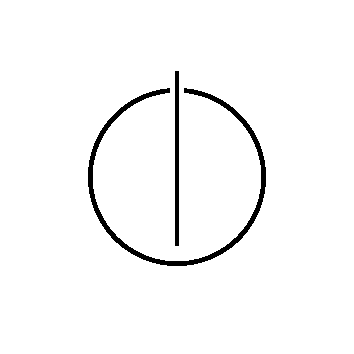
\includegraphics[width=4cm]{styles/informat.png}
  \end{figure}
  
  \end{center}
%	\clearemptydoublepage
%	
%	% The titlepage for the CAMP report document.
% Included by MAIN.TEX


%--------------------------------------------------
% The title page
%--------------------------------------------------

% correct BCOR - undo at the end !!!
\def\bcorcor{0.15cm}
\addtolength{\hoffset}{\bcorcor}

\thispagestyle{empty}

 \vspace{10mm}
\begin{center}
	       \oTUM{4cm}
	   
	   \vspace{5mm}     
	   \huge FAKULT{\"A}T F{\"U}R INFORMATIK\\ 
	   \vspace{0.5cm}
	 \large DER TECHNISCHEN UNIVERSIT{\"A}T M{\"U}NCHEN\\
        
	\end{center}
		

\vspace{10mm}
\begin{center}

   {\Large \doctype}

  \vspace{10mm}
  
  {\LARGE \title}\\
  
  
  \vspace{10mm}
  
  
  {\LARGE  \titleGer}\\
  
  
  \vspace{10mm}

    %\hfill
    \begin{tabular}{ll}
	   \Large Author:     & \Large \author \\[2mm]
	   \Large Supervisor:    & \Large Prof. Dr. Claudia Eckert\\[2mm]				
	   \Large Advisor:	& \Large M.Sc. Paul-Ioan Muntean\\[2mm]
	   \Large Date:       & \Large November 15, 2015
	 \end{tabular}
	 
	 \vspace{5mm}
	 
	 \begin{figure}[h!]
  \centering
   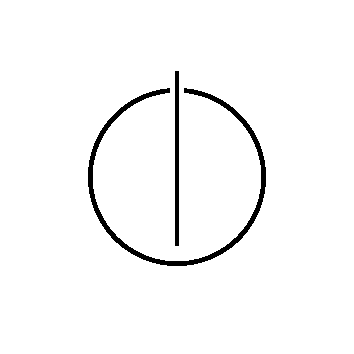
\includegraphics[width=4cm]{styles/informat.png}
  \end{figure}
   

\end{center}

% undo BCOR correction
\addtolength{\hoffset}{\bcorcor}
	
	
%	\input{components/cover_maschmeyer}
	\clearemptydoublepage
	
	% The titlepage for the CAMP report document.
% Included by MAIN.TEX


%--------------------------------------------------
% The title page
%--------------------------------------------------

% correct BCOR - undo at the end !!!
\def\bcorcor{0.15cm}
\addtolength{\hoffset}{\bcorcor}

\thispagestyle{empty}

 \vspace{10mm}
\begin{center}
	       \oTUM{4cm}
	   
	   \vspace{5mm}     
	   \huge FAKULT{\"A}T F{\"U}R INFORMATIK\\ 
	   \vspace{0.5cm}
	 \large DER TECHNISCHEN UNIVERSIT{\"A}T M{\"U}NCHEN\\
        
	\end{center}
		

\vspace{10mm}
\begin{center}

   {\Large \doctype}

  \vspace{10mm}
  
  {\LARGE \title}\\
  
  
  \vspace{10mm}
  
  
  {\LARGE  \titleGer}\\
  
  
  \vspace{10mm}

    %\hfill
    \begin{tabular}{ll}
	   \Large Author:     & \Large \author \\[2mm]
	   \Large Supervisor:    & \Large Prof. Dr. Claudia Eckert\\[2mm]				
	   \Large Advisor:	& \Large M.Sc. Paul-Ioan Muntean\\[2mm]
	   \Large Date:       & \Large November 15, 2015
	 \end{tabular}
	 
	 \vspace{5mm}
	 
	 \begin{figure}[h!]
  \centering
   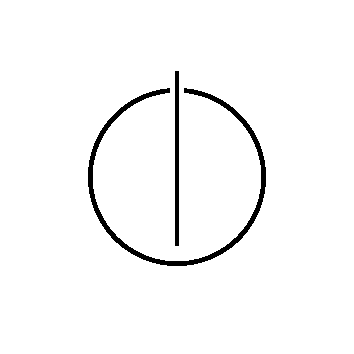
\includegraphics[width=4cm]{styles/informat.png}
  \end{figure}
   

\end{center}

% undo BCOR correction
\addtolength{\hoffset}{\bcorcor}
	
	
	\clearemptydoublepage


\thispagestyle{empty}
\selectlanguage{german}
	\vspace*{0.8\textheight}
	\noindent
	Ich versichere, dass ich diese Diplomarbeit selbst{\"a}ndig verfasst und nur 
	die angegebenen \\Quellen und Hilfsmittel verwendet habe.
	
	\vspace{15mm}
	\noindent
	M{\"u}nchen, den \today \hspace{5cm} \author
\selectlanguage{english}
\newpage
	
	\clearemptydoublepage
\phantomsection
\addcontentsline{toc}{chapter}{Acknowledgements}	


%\chapter*{Acknowledgements}

\vspace*{2cm}

\begin{center}
{\Large \bf Acknowledgments}
\end{center}

\vspace{1cm}




I would like to express my deepest appreciation to all those who provided me the possibility to complete this thesis. A special gratitude and thanks I give to my supervisor Prof. Dr. Claudia Eckert and my advisor, MSc. Paul Muntean, whose guidance, stimulating suggestions and encouragement, helped me in all the time of research and writing of this thesis. Without their cooperation in the last 6 months, this thesis could not be done smoothly.

Last but not the least, I wish to thank my family for their support and encouragement throughout my Master study.
	
	% Abstract for the TUM report document
% Included by MAIN.TEX


\clearemptydoublepage
\phantomsection
\addcontentsline{toc}{chapter}{Abstract}	





\vspace*{2cm}
\begin{center}
{\Large \bf Abstract}
\end{center}
\vspace{1cm}

Information flow vulnerabilities detection with static code analysis techniques is challenging because code
is usually not available during the software design phase and
previous knowledge about what should be annotated and tracked
is needed. To detect information flow errors in UML state
charts and C code are not easy task as they can cause data leakages or unexpected program behavior. In this research it is proposed that textual annotations used to
introduce information flow constraints in UML state charts and code which are afterwards automatically loaded by information flow checkers that check if imposed constraints hold or not. The experimental results on selected sample scenarios shows that this approach
is effective and can be further applied to other types of UML
models and programming languages as well, in order to detect
different types of vulnerabilities.

The contributions of this thesis is the development of a system for semi-automated detection of sanitization, authentication and declassification errors in UML state charts. A light-weight security annotation language is used in order to define information flow constraints regarding authentication, declassification and santization function errors  in UML state charts and source code.  Annotation language editor is designed as eclipse
plug-ins which is used to edit UML state charts and
source code files. Developed Source code generator as eclipse plug-in which is used to generate C code with header files from UML State chart. And finally experimented automatic loading and usage of textual annotations inside 3 new checkers.

	\tableofcontents
  
  \clearemptydoublepage

\phantomsection
\addcontentsline{toc}{chapter}{Outline of the Thesis}

\begin{center}
	\huge{Outline of the Thesis}
\end{center}


%--------------------------------------------------------------------
%\section*{Part I: Introduction and Theory}

\noindent {\scshape Chapter 1: Introduction}  \vspace{1mm}

\noindent  This chapter presents an overview of the thesis and it's purposes. 

\noindent {\scshape Chapter 2: Background}  \vspace{1mm}

\noindent  This chapter describes the background informations and the essential theories needed for our research. Authentication, declassification and sanitization functionalities are also presented with example in this chapter. Scientific fundamentals 

%--------------------------------------------------------------------
%\section*{Part II: Implementation and Analysis}

\noindent {\scshape Chapter 3: Challenges and Annotation Language Extension}  \vspace{1mm}

\noindent  This chapter presents the challenges and annotation language extension for the system. Annotation language extension process, what technology and tools are used to develop and how it works are also presented inside this chapter.

\noindent {\scshape Chapter 4: Implementation}  \vspace{1mm}

\noindent  This chapter presents the implementation of the system. Implementation mechanism, technology and tools which have been used to develop the system are also presented inside this chapter.

\noindent {\scshape Chapter 5: Experiments}  \vspace{1mm}

\noindent  This chapter presents the different application areas of the system. Inside this chapter the system is checked for three real-life scenarios and presented the outcome of the system. 

\noindent {\scshape Chapter 6: Related Work}  \vspace{1mm}

\noindent  This chapter presents some of the related work of this research. Some of the related tools that have been already developed and comparison with them are also presented inside this chapter.


%--------------------------------------------------------------------
%\section*{Part III: Conclusion and Future Works}

\noindent {\scshape Chapter 7: Limitations, Conclusion and Future Work}  \vspace{1mm}

\noindent  This chapter presents the limitations of this research, conclusion of the whole research along with future work intentions.

	\mainmatter
	
	
		% ---------------------------------------------------------------------------
		%
		%Introduction and Background Theory
		%
		% ---------------------------------------------------------------------------
		\part[Introduction and Theory]{Introduction and Theory}
		\label{part:introAndBackgroundTheory}
		\chapter{Introduction}
\label{chapter:Introduction}

The detection of information flow vulnerabilities uses dynamic analysis techniques , static analysis techniques and hybrid techniques which combine static and dynamic approaches. The static techniques need to know when to use  sanitization , declassification and authentication functions.
A solution for tagging sanitization, declassification and authentication in source code is based on libraries which contain all needed annotations attached to function declarations. This approach plays an important role mainly for static analysis bug detection techniques where the information available during program run-time is not available nor the interaction with the environment can be fully simulated.
Extended Static Checking (ESC) is a promising research area which tries to cope with the shortage of not having the program run-time information. During extended static analysis additional information is provided to the static analysis process. This information can be used to define trust boundaries and tag variables. Textual annotations are usually manually added by the user in source code. At the same time annotations can be automatically generated and inserted into source code . ESC can be used to eliminate bugs in a late stage of the software project when code development is finished. Tagging and checking for information exposure bugs during the design phase would eliminate the potential of implementing software bugs which can only be removed very costly after wards. Thus security concerns should be enforced into source code right after the conceptual phase of the project.
The paper presents five challenges concerning ESC. The last challenge reports of the annotation as being a very time consuming burden and is therefore disliked by some programming
teams. The authors argue about the fact that annotations can cover design decisions and enhance the quality of source code. We argue that annotations are necessary in order to do ESC and the user needs a kind of assistance tool that helps selecting the suited annotation based on the current context. Thus the annotation burden needed for learning and applying the language should be reduced. At the same time adding annotations to reusable code libraries reduces even more the annotation burden since libraries can be reused, shared and changed by software development
teams.\\

Information flow errors in UML models
and code are introduced by software designers or programmers
who are sometimes blind with respect to the fact that they
are trained to focus point-wise (one code line and one data flow
at a time). This is why it is important to develop techniques
and tools which can detect this type of errors before they
materialize in production code.Information flow vulnerabilities are hard to detect because static code analysis techniques need previous knowledge about what should be considered a security issue. Code annotations which are added mainly during software development [6] can be used to provide additional knowledge regarding security
issues. On the other hand code annotations can increase the
number of source code lines by 10% [27]. In order to detect
information flow vulnerabilities software artifacts have to be
annotated with annotations attached to public data, private data and to system trust boundaries. Next, annotated artifacts have
to be made tractable by tools which can use the annotations
and check if information flow constraints hold or not based on
information propagation techniques.\\

The detection of information flow vulnerabilities in code
and UML state charts is not well addressed and is particularly
challenging. Foremost, there is no common annotation language for annotating UML state charts and source code with
information flow security constraints such that errors can be
detected also when code is not available. Second, there are
no automated checking tools which can reuse the annotated
constraints in early stages of software development to check
for information flow errors. We think that it is important to
specify security constraints as early as possible in the software
development process in order to avoid later costly repairs or
exploitable vulnerabilities.
 
\section{Latex Introduction}
There is no need for a latex introduction since there is plenty of literature out there.
 



		\chapter{Background Information}

\section{Sanitization}
Sanitization is the process of removing sensitive information from a document or other message or sometimes encrypting messages, so that the document may be distributed to a broader audience. Sometimes sanitization can be called as an operation that ensures that user input can be safely used in an SQL query. Web applications use malicious input as part of a sensitive operation without having properly checked or sanitized the input values from the user. Previous research on vulneribility analysis has mostly focused on identifying cases which web applications directly uses external input for critical operations. It is suggested that always use proper sanitization method to validate external input values from the user for any application.For example, user inputs must always flow through a sanitizing function before flowing into a SQL query or HTML, to avoid SQL injection or cross-site scripting vulnerabilities.\\

Reflection of security breaches are very significant for high assurance system. For examples of this type of systems are aircraft navigation, where a fault could lead to a crash, various control systems which has critical infrastructure , where an error 
could cause toxic waste to leak, and weapons targeting, where an inaccuracy could result in severe collateral damage. In such
operational environments, the impact is virtually irreversible and must therefore be prevented even if it is likely to occur
with low probability.It's always good that transforming information to a form which is suitable for release or sanitize the information by redacting some portions of it.\\

Three of the top five most common website attacks are SQL injection, cross-site scripting (XSS), and remote file inclusion (RFI). The root cause of these attacks is common: input sanitization. All three exploits are leveraged by data sent to the web server by the end user. When the end user is a good guy, the data he sends the server is relevant to his interaction with the website. But when the end user is a hacker, he/she can exploit this mechanism to send the web server input which is deliberately constructed to escape the legitimate context and execute unauthorized actions.\\

Input sanitization describes cleansing and scrubbing user input to prevent it from jumping the fence and exploiting security holes. But thorough input sanitization is hard. While some vulnerable sites simply don't sanitize at all, others do so incompletely, lending their owners a false sense of security.\\

Some basic purpose of sanitization are given below:
\begin{itemize}
	\item Remove malicious elements from the input.
	\item To identify the set of parameters and global variables which must be sanitized before calling functions.
	\item It is acceptable to first pass the untrusted user input through a trusted sanitization function.	
	\item Any user input data must flow through a sanitization function before it flows into a SQL query.
	\item Confidential data needs to be cleansed to avoid information leaks.
	\item Most paths that go from a source to a sink pass through a sanitizer.
	\item Developers typically define a small number of sanitization functions in libraries.
	\item Prevent web attacks using input sanitization.
\end{itemize}

\section{Declassification}
Information security has a challenge to address: enabling information flow controls with expressive information release (or declassification) policies. In a scenario of systems that operate on data with different sensitivity levels, the goal is to provide security assurance via restricting the information flow within the system. Practical security-typed languages support some form of declassification through which high-security information is allowed to flow to a low-security system or observer.\\

United States Federal Trade Commission reveals the damage that is continually caused by electronic information leakage. In protecting sensitive information, including everything from credit card information to military secrets to personal, medical information, there is a highly
need for software applications with strong, confidentiality guarantees.
Security-typed languages promise to be a valuable tool in making provably secure software applications. In such languages, each
data item is labeled with its security policy. In practical security-typed languages support some form of declassification, in which high-security information is permitted to flow to a low-security receiver/observer \\

To declassify information means lowering the security classification of selected information. Sabelfeld and Sands \cite{ref_3_sabelfeld2009declassification} identify four different dimensions of declassification, what is declassified, who is able to declassify, where the declassification occurs and when the declassification takes place.\\

Myers and Liskov introduced the decentralized label model \cite{ref_4_myers2000protecting}, describing how labels could be applied
to a programming language and then used to check information
flow policy compliance in distributed systems. The framework
includes a declassify function for downgrading data if the
owners policies allow. The model allows principals to define their own downgrading policies.\\

\subsection{Dimensions of declassification}
Classification of the basic declassification goals according to four axes: what information is released, who releases information, where in the system information is released and when information can be released.

\begin{itemize}
   \item What : Selective or Partial information flow policies \cite{ref_5_cohen1977information,ref_6_cohen1978information,ref_7_joshi2000semantic,ref_8_giacobazzi2005adjoining} regulate what
   information may be released. Partial release guarantees that only a part of a secret is
   released to a public domain. Partial release can be specified in terms of precisely which
   parts of the secret are released. This is useful,
   for example, when partial information about a credit card number or a social security number is used for logging.
   
   \item Who : In a computing system it is essential to specify who controls information release .
   Ignoring the issue of control opens up attacks where the attacker hijacks release
   mechanisms to launder secret information. Myers and Liskov decentralised label
   model \cite{ref_9_myers1997decentralized} security labels with explicit ownership information. According to this approach, information release of some data is safe if it is performed by the
   owner who is explicitly recorded in the data security label. This model has been used for enhancing Java with information flow controls \cite{ref_10_myers1999jflow} and has been implemented in
   the Jif compiler \cite{ref_11_myers2001jif}.
   
   \item Where : In a system information  Where is an important aspect of information release.One can ensure that no other  part can release further information.
   by delegating particular parts of the system to release information.Declassification
   via encryption is not harmful as long as the program is, in some sense, noninterfering
   before and after encryption.  A combination of \enquote{where} and \enquote{who} policies in the presence of encryption has
   been recently investigated by Hicks et al.\cite{ref_12_hicks2005declassification}
   
   \item When : The fourth dimension of declassification is  \enquote{when} information should be released.The work of Giambiagi and Dam \cite{ref_19_giambiagi2003secure} focuses on the correct implementation of security protocols. Here the goal is not to prove a noninterference property of the protocol, but to use the components of the protocol description as a specification of what and when information may be released.Chong and Myers security policies \cite{ref_13_chong2004security} address when information is released.By annotating variables this is achieved.
   
\end{itemize}

For a given model, the \enquote{what} and \enquote{when} dimensions seem relatively straightforward to define formally. The \enquote{what} dimension abstracts the extensional semantics
of the system; the \enquote{when} dimension can be distinguished from this since it requires an intensional semantics that (also) models time, either abstractly in terms of complexity
or via intermediate events in a computation. The \enquote{who} and \enquote{where} dimensions are
harder to formalize in a general way, beyond saying that they cannot be captured by the
\enquote{what} and \enquote{when} dimensions.

\section{Authentication}
Authentication is the mechanism which confirms the identity of users trying to access a system. For a user to be granted access to a resource, they must first prove that they are who they claim to be. Generally this is handled by passing a key with each request (often called an access token, User verification using user id and password). The system or server verifies that the access token or user id and password is genuine, that the user does indeed have the required privileges to access the requested resource and only then the request granted.\\
Also authentication can be defined as it is the process by which the system validates a user's logon information. A user's name and password are compared to an authorized list and if the system detects a match then access is granted to the extent specified in the permission list for that user.\\

One familiar use of authentication and authorization is access control. A computer system that is supposed to be used only by those authorized must attempt to detect and exclude the unauthorized. Common examples of access control involving authentication include:
\begin{itemize}	
	\item A computer program using a blind credential to authenticate to another program.
	\item Logging in to a computer.	
	\item Using an Internet banking system.
	\item Withdrawing cash from an ATM and more
	\item Assurance of identity of person or originator of data.
\end{itemize}

 A variety of authentication technologies have hit the market over the years.To better understand what they are and how they compare to the user name/password combination, it helps to be familiar with the standard authentication factors something you know, something you have and something you are and how each technology leverages them to power its authentication capabilities.
 \begin{itemize}	
	\item Something you know is a bit of knowledge committed to memory, such as a password or
	 an answer to a secret question.
	\item Something you have is an item that is owned or carried, such as a smart card or similar
	 hardware device.
	\item	 Something you are is a physical attribute that can be identified, such as a fingerprint or voice.
\end{itemize}

According to the networkworld \cite{ref_21_networld} now-a-days seven strong authentication methods are:
\begin{itemize}
\item Computer recognition software.
\item Biometrics
\item E-mail or SMS one-time password (OTP).
\item One Time Password (OTP) token.
\item Out of band.
\item Peripheral device recognition.
\item Scratch-off card.
\end{itemize}	


\section{ Detecting Information Flow Errors During Design:}
If a step of function call like authentication, sanitization or declassification is missing inside the program then this can lead to software vulnerabilities. In the figure \ref{figure_FunctionCallMissing} left side picture depicted that it has three functions. Among them func2() is named either sanitization/declassification/authentication function. Which means in this scenario there will be no error regarding sanitization/declassification/authentication function. On the other hand the right side picture represents there is a missing function of sanitization/declassification/authentication function. That's why it is the buggy path of UML state charts during design stage of software life cycle. 
\begin{figure}[htbp]
	\centering
	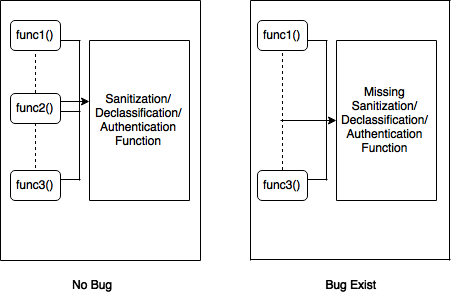
\includegraphics{styles/FunctionCallMissing.png}
	\caption{Information flow errors during design}
	\label{figure_FunctionCallMissing}
\end{figure}


\section{ Detecting Information Flow Errors During Coding:}

Figure \ref{figure_bug_detection_during_coding} depicts two explicit information flows according to A lattice model of secure information flow of Denning \cite{ref_14_denning1976lattice} contained in two systems (system 1) and (system 2)
where each of the flows starts with statement variable a and ends with leaving the system. The the variable declaration up to outside the system represent C language statements. System 1 is depicted in left side containing the flow from the source to the sink and leaving the system indicated with circles at the top and bottom of each of the
two information flows. A source is any function or programming language statement which provides private information through a system boundary. A sink can be a function call or programming language statement which exposes private information to the outside of the system through a system boundary. A system boundary can be a statement, function call, class, package or module. In figure 2.2 the source and sink represent C language statements where information enters and respectively leaves system 1 or system 2. The variable a was tagged with label \enquote{H} (confidential) as it inserts confidential information into system 1. The arrows represent the passing of the confidential label \enquote{H} between the program statements. When a variable labeled with \enquote{H} is about to leave system 1 or system 2 without passing through either authentication/declassifiaction/sanitization function then a bug report should be created.In figure 2 right side system has a bug because it passes a secured/confidential information without passing through authentication/declassifiaction/sanitization function. These functions either authenticated,declassified or sanitized  secured/confidential information and makes the variable label as \enquote{L} to leave the system. But in the left part of the picture there is no bug as in this system, secured/confidential information and the variable which is labeled with \enquote{H} passes through either authentication/declassifiaction/sanitization function.

\begin{figure}[htbp]
	\centering
	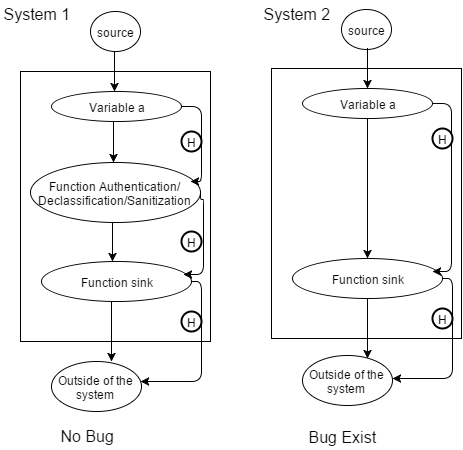
\includegraphics{styles/bug_detection_during_coding.png}
	\caption{Information flow errors during coding}
	\label{figure_bug_detection_during_coding}
\end{figure}

		
		
		
		%
		%% ---------------------------------------------------------------------------
		%%
		%% Fully Automated Calibration for Ultrasound
		%%
		%%% ---------------------------------------------------------------------------
		\part[The 2nd Part]{The Second Part}
		\label{part:secondP}
		
		
		% ---------------------------------------------------------------------------
		%
		% Appendix
		%
		% ---------------------------------------------------------------------------
		
		\part*{Appendix}
		\addcontentsline{toc}{part}{Appendix}
		
		\appendix %---------------------------------------
		
		\chapter{Appendix}
\section{Appendix A: Source Code Editor with Annotation Language}
\lstinputlisting[numbers=left,firstnumber=1,firstline=1]{sourceCode/MyDsl.xtext}

\section{Appendix B: C Code Generator}	

	\lstinputlisting[numbers=left,firstnumber=1,firstline=1]{sourceCode/Naming.xtend}
	
	\lstinputlisting[numbers=left,firstnumber=1,firstline=1]{sourceCode/Types.xtend}
	
\section{Appendix C: Three Checkers in Static Analysis Engine}

\section{Appendix D: Sequence Diagram Generator}

		
	


  \clearemptydoublepage
  
	\bibliography{bibliography/literature}
	
 
\end{document}

